% !TeX spellcheck = it_IT
\newpage
\section{Assembler}
\subsection{Numeri frazionari}
Supponiamo di avere il numero $2.375_{10}$. Per convertirlo in base 2, prima convertiamo la parte intera ($2=10$) e poi la parte frazionaria:
\begin{equation*}
	\begin{split}
		2.375_{10} = 10.011 \\
		0.375 \cdot 2 = 0.75 \\
		0.75 \cdot 2 = 1.5 \\
		0.5 \cdot 2 = 1 \\
	\end{split}
\end{equation*}
Per fare la conversione inversa:
\begin{equation*}
	10.011 = 1*2^1 + 1 * 2^{-2} + 1 * 2^{-3}=2+\frac{1}{4} + \frac{1}{8} = 2.375
\end{equation*}
\subsubsection{Virgola fissa}
\subsubsection{Virgola mobile}
Lo standard IEEE 754 divide i numeri in due categorie:
\begin{itemize}
	\item \textbf{Singola precisione}
	\item \textbf{Doppia precisione}
\end{itemize}

\newpage
\subsection{Mappa di memoria}
\begin{wrapfigure}{r}{0.25\textwidth}
	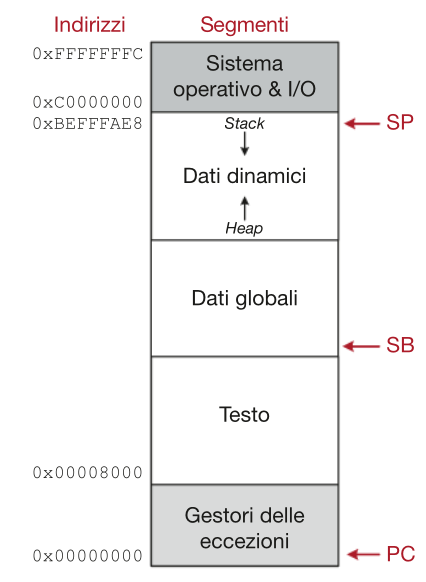
\includegraphics[scale=0.3]{arm_memory.png}
\end{wrapfigure}
ARM utilizza indirizzi a $32$ bit e di conseguenza ha $2^{32}$ byte di spazio di indirizzamento. Gli indirizzi di parola sono a multipli di $4$. Lo spazio viene diviso in cinque segmenti.
\subsubsection{Testo}
Contiene il programma il linguaggio macchina. È a \textbf{sola lettura} e può contenere anche delle costanti dette \textit{literal}.
\subsubsection{Dati globali}
Memorizza le variabili che sono accessibili da tutto il programma e che sono in \textbf{lettura/scrittura}. Si accede a queste variabili a partire da un indirizzo base statico che punta all'inizio del segmento, per convenzione \textit{R9}, chiamato \textbf{SB}.
\subsubsection{Dati dinamici}
Contiene \textbf{stack} e \textbf{heap}. I dati qui vengono allocati e deallocati dinamicamente durante l'esecuzione del programma.
\begin{itemize}
	\item \textbf{Stack}: \textit{SP} viene inizializzato con l'indirizzo in cima al segmento in quanto poi cresce verso il basso (LIFO). Contiene dati temporanei e variabili locali che sono troppo grandi per stare nei registri. Viene anche usato per salvare e ripristinare i registri.
	\item \textbf{Heap}: memorizza i dati allocati dal programma durante le esecuzioni. Qui gli elementi possono essere salvati ed eliminati in qualsiasi ordine. Cresce verso l'alto a partire dall'inizio del segmento
\end{itemize}
Per evitare che \textit{stackj} e \textit{heap} si sovrappongano con conseguente perdita di dati, il programmatore deve assicurasi di lanciare errori di tipo \textit{out-of-memory}.
\subsubsection{Eccezioni, OS, I/O}
Contiene il vettore delle eccezioni e i gestori delle eccezioni. Oltre che il sistema operativo e l'ingresso/uscita mappato in memoria.

\subsection{Codifica}
Le istruzioni ARM sono codificate in $32$ bit che ha un formato variabile in base al tipo di istruzione da eseguire.
\subsubsection{Elaborazione dati}
\begin{center}
	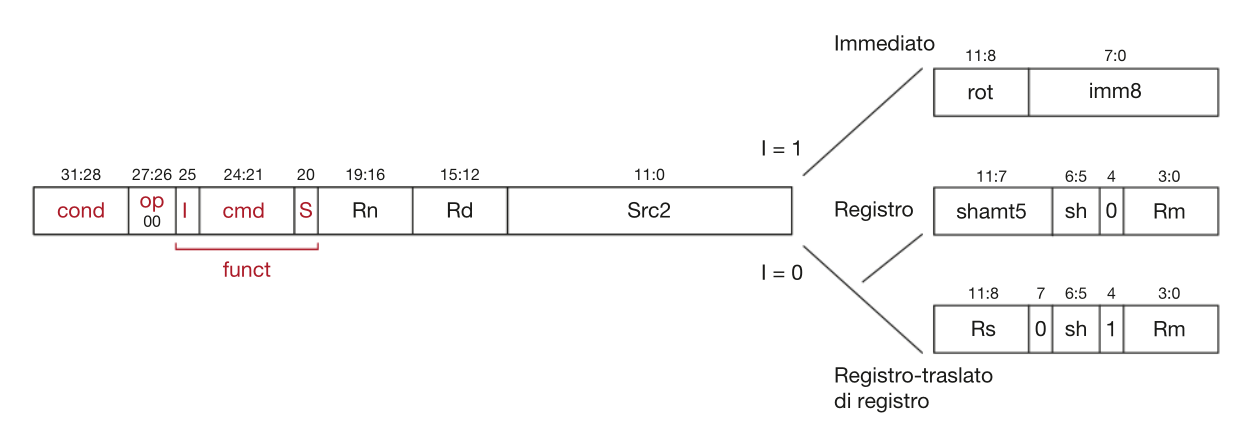
\includegraphics[scale=0.35]{arm_elab.png}
\end{center}
\begin{observation}
	\label{obs:rapp_rot}
	Le istruzioni di elaborazione dati hanno una rappresentazione basata su un \textit{immediato} \textbf{imm8} ruotato a destra di $2 \cdot \mathbf{rot}$. Questo permette di codificare in maniera comoda molte costanti utili, come piccole potenze di due, in pochi bit.
\end{observation}
Vediamo lo scopo di ogni campo:
\begin{itemize}
	\item \textbf{cond}: \textit{condition}, identifica l'eventuale condizione da aggiungere all'istruzione. Se non ve ne sono $cond=1110_2$ \label{it:cond}
	\item \textbf{op}: \textit{OPeration CODE}, che nel caso delle operazioni di elaborazione dati $op = 00_2$
	\item \textbf{funct}: \textit{function}, identifica l'istruzione
	\begin{itemize}
		\item \textbf{I}: vale $1$ quando \textit{Src2} è un immediato
		\item \textbf{cmd}: valore specifico per ogni istruzione
		\item \textbf{S}: vale $1$ quando l'istruzione modifica le flag di condizione
	\end{itemize}
	\item \textbf{Rn}: registro del primo operando sorgente \label{it:rn}
	\item \textbf{Rd}: registro destinazione \label{it:rd}
	\item \textbf{Src2}: registro del secondo operando sorgente
	\begin{itemize}
		\item \textit{Immediato}:
		\begin{itemize}
			\item \textbf{rot}: vedi \ref{obs:rapp_rot}
			\item \textbf{imm8}: vedi \ref{obs:rapp_rot}
		\end{itemize}
		\item \textit{Registro traslato di una costante}:
		\begin{itemize}
			\item \textbf{shamt5}: immediato da utilizzare per la traslazione
			\item \textbf{sh}: indica il tipo di traslazione da effettuare \label{it:sh}
			\item \textbf{Rm}: registro di partenza \label{it:rm}
		\end{itemize}
		\item \textit{Registro traslato del contenuto di un altro registro}:
		\begin{itemize}
			\item \textbf{Rs}: registro che contiene il valore per effettuare la traslazione
			\item \textbf{sh}: vedi \hyperref[it:sh]{prima}
			\item \textbf{Rm}: vedi \hyperref[it:rm]{prima}
		\end{itemize}
	\end{itemize}
\end{itemize}

\subsubsection{Accesso alla memoria}
\begin{center}
	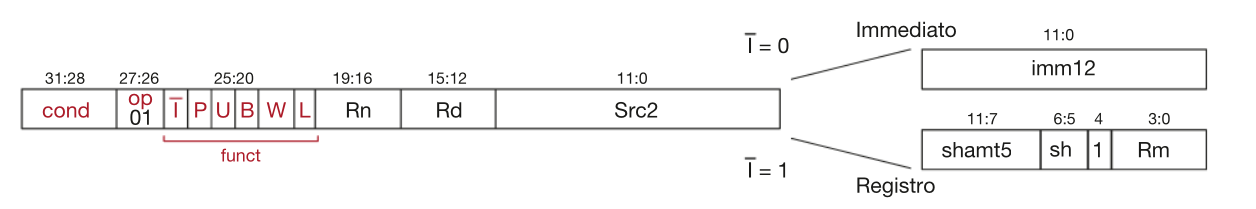
\includegraphics[scale=0.35]{arm_mem.png}
\end{center}
\begin{itemize}
	\item \textbf{op}: nel caso delle operazioni di accesso alla memoria dati$op = 01_2$
	\item \textbf{funct}: \textit{function}, identifica l'istruzione
	\begin{itemize}
		\item \textbf{$\bar{I}$}: indica se lo spiazzamento è un immediato o un registro
		\item \textbf{U}: indica se lo spiazzamento deve essere sommato o sottratto
		\item \textbf{L e B}: indicano il tipo di accesso alla memoria
		\begin{table}[!h]
			\centering
			\begin{tabular}{|c|c|c|}
				\hline
				\textbf{L} & \textbf{B} & \textbf{Istruzione}\\
				\hline
				0 & 0 & \textit{STR} \\
				0 & 1 & \textit{STRB}\\
				1 & 0 & \textit{LDR} \\
				1 & 1 & \textit{LDRB} \\
				\hline
			\end{tabular}
		\end{table}
		\item \textbf{P e W}: indicano in che modo gestire l'indice
		\begin{table}[!h]
			\centering
			\begin{tabular}{|c|c|c|}
				\hline
				\textbf{P} & \textbf{W} & \textbf{Modi di gestione}\\
				\hline
				0 & 0 & Post-indice \\
				0 & 1 & Non supportato \\
				1 & 0 & Spiazzamento \\
				1 & 1 & Pre-indice \\
				\hline
			\end{tabular}
		\end{table}
	\end{itemize}
	\item \textbf{Src2}: definisce l'offset
	\begin{itemize}
		\item \textit{Immediato}: \textbf{imm12}, unsigned a $12$ bit
		\item \textit{Registro traslato di una costante}
	\end{itemize}
\end{itemize}

\subsubsection{Salto}
\begin{center}
	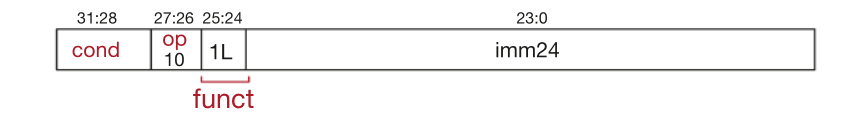
\includegraphics[scale=0.35]{arm_branch.png}
\end{center}
\begin{itemize}
	\item \textbf{op}: nel caso delle operazioni di accesso alla memoria dati$op = 10_2$
	\item \textbf{funct}: due bit, di cui il più significativo è sempre $1$ e l'altro è \textbf{L}, ovvero il tipo di salto:
	\begin{itemize}
		\item $1$ per \textit{BL}
		\item $0$ per \textbf{B}
		\item \textbf{U}: indica se lo spiazzamento deve essere sommato o sottratto
	\end{itemize}
	\item \textbf{imm24}: indirizzo di destinazione del salto scritto come differenza con $PC + 8$ 
\end{itemize}
\subsubsection{Literal}
Quando è necessario caricare dei \textit{literal} a $32$ bit, non si può usare \textit{MOV} dato che prende una sorgente a $12$ bit. Si usa quindi:
\begin{lstlisting}[language={[x86masm]Assembler}]
	LDR Rd, =literal
	LDR Rd, =label
\end{lstlisting}
che può prendere o una costante (literal) o un indirizzo ad una zona di memoria contenente il literal (label). In entrambi i casi il valore viene salvato nel \textbf{serbatoio dei literal} nel segmento \textit{testo} della memoria. Questo deve stare a meno di $4096$ byte di distanza dall'istruzione LDR in modo che il caricamento si possa eseguire correttamente. Di conseguenza il programma deve evitare il serbatoio e non considerarlo come istruzioni.

\subsubsection{NOP}
Istruzione che non fa nulla, tradotta come:
\begin{lstlisting}[language={[x86masm]Assembler}]
	MOV R0, R0
\end{lstlisting}
Può servire per introdurre ritardi e allineare istruzioni.